\documentclass[10pt,a4paper,twoside]{article}
\usepackage{amsfonts}
%\usepackage{ICDD}

\usepackage[utf8]{inputenc}
\usepackage[T1]{fontenc}

\usepackage{graphicx}
\usepackage{float}
\usepackage{multirow}

\makeatletter
    \def\thebibliography#1{\section*{References\@mkboth
      {REFERENCES}{REFERENCES}}\list
      {[\arabic{enumi}]}{\settowidth\labelwidth{[#1]}\leftmargin\labelwidth
    \advance\leftmargin\labelsep
    \usecounter{enumi}}
    \def\newblock{\hskip .11em plus .33em minus .07em}
    \sloppy\clubpenalty4000\widowpenalty4000
    \sfcode`\.=1000\relax}
    \makeatother

%\addtolength{\oddsidemargin}{1.3cm}
%\addtolength{\evensidemargin}{-0.1cm}
\setlength{\topmargin}{-0.2cm}
%\setlength{\textheight}{20cm} \setlength{\textwidth}{13cm}
\setlength{\textheight}{8.890in} \setlength{\textwidth}{6.3in}
\setlength{\oddsidemargin}{.077in}
\setlength{\evensidemargin}{.077in} \thispagestyle{empty}

\begin{document}
%\tableofcontents
\pagestyle{empty}

\def\SHORTTITLE  {Secured Bootloader}%

\vspace*{3cm}
%\antet
\markboth{\hfill  Barbu Paul - Gheorghe}{\hfill
\SHORTTITLE}

\begin{center}
{\Large \bf Secured Bootloader: application for initializing and updating microcontroller applications}
\par\vspace*{0.5cm}
{\bf Barbu Paul - Gheorghe }
\end{center}

\vspace*{0.3cm}
%%%%%%%%%%%%%%%%%%%%%%%%%%
%%%%%% PROOF.TEX %%%%%%%%%
%%%%%%%%%%%%%%%%%%%%%%%%%%
\tolerance 10000
\newtheorem{theorem}{Teorem\check{a}}
\newtheorem{lemma}{Lema}
\newtheorem{definition}{Definitie}
\newtheorem{example}{Exemplu}
\newtheorem{xca}{Exercitiu}
\newtheorem{remark}{Observatie}
\newtheorem{proposition}{Propozitie}
\newtheorem{corollary}{Corolar}

%Please use these definitions for Latex entities (theorem, lemma, etc.)
%If you need other definitions add to this list and notify us, by e-mail, about this.
%--------------------------------------

\begin{abstract}
This paper aims to create a bootloader for embedded devices. The purpose of the bootloader is to be the first to run when the microcontroller starts and to provide a way of controlling what application runs next, similarly to how bootloaders work on the desktop systems.
The difference here being that the bootloader's purpose is to allow the embedded device to be much more flexible, since the application running on the microcontroller can be changed without using specialized hardware. This flexibility and the fact that no specialized hardware programmers are needed also leads to a reduction of costs for deploying and maintaining the embedded systems. These two goals, flexibility and cost reduction must be accompanied by a third one: security. The recent growth of embedded systems in the IoT (Internet of Things) domain demands that the device deployed be more secure than in the past.
\end{abstract}

\section{Introduction}
Working in an embedded area we have to think about how we can achieve the goals that we've set for the bootloader application.

First of all, any microcontroller that has to be programmed must be connected to a desktop system using a specialized piece of hardware, called most commonly a "programmer device", also known as a JTAG connector \cite{jtag}. Through this connector the developer of the application can perform the flashing of the application.
This is the first point that the application developed in this article will tackle, the fact that an expensive hardware tool is needed for flashing most industrial microcontrollers. This issue will be solved by allowing the bootloader application to communicate through the microcontroller's RS232 port. Hence we will develop a serial protocol for writing applications on the embedded device. According to the goals set, this protocol also has to be secure, when flashing an application on the microcontroller the flashed application's machine code should not be available to the outside world.

The bootloader’s role is to allow the developer to flash a new application on an MCU without having to connect a JTAG device to it. This also allows for a simpler flashing procedure that the client can also perform when there is a need for a firmware upgrade. The bootloader loads applications only via RS232 and only in a specific, encrypted file format. Hence, the bootloader makes sure that the flashed application is not tampered with by third parties, in which case it should refuse to boot the application. For security reasons in order to upgrade the bootloader a classical flashing process needs to be used, eg. JTAG.
The classical use case for the bootloader is when a client has devices all over the world and a firmware upgrade is necessary, then the client’s technicians can perform the upgrade by themselves, using the bootloader and the new firmware file received from the developer. This is done in order to avoid bringing in all the devices and flashing them at headquarters, then shipping them back to their client's locations.
In order for the bootloader to work properly it should receive via RS232 a valid firmware file (.fw extension).
This has to be created by an application, which should also be responsible for encrypting it, we'll call this application "Bundler", since it creates an encrypted file that will contain the application that the bootloader will load on a microcontroller. In order for the client to be able to program the microcontroller and to use the bootloader he will need an application that will send the firmware file to the MCU, via the serial port, we will call this tool the "Flasher", since it does the flashing of the application, similar to the classical process of programming a microcontroller using a JTAG connector.

\section{How does a bootloader work?}
A bootloader can be found on any system that needs to load an operating system or, in our case, a third party application. The etimology of this word stems from the word "to bootstrap", which means "to pull oneself up by one's bootstraps" \cite{bootstrapping}.

A bootloader is, without exception, the first application that runs on a system. It is loaded in memory (in RAM - Random Access Memory) from non-volatile storage, such as hard-disks or, in the case of microcontrollers, flash memory. After loading, the bootloader (on x86 systems) generally asks the user what operating systems he wants to load. On embedded devices, this usually cannot happen because a microcontroller, by default has reduced input and output capabilities. Also a key difference on the embedded side of things is the fact that a microcontroller has a smaller non-volatile memory than a personal computer has and this allows only one application to be stored at a time on the microcontroller, so the bootloader, after start-up, will automatically choose just this application.
But since one of our goals is to allow the user to change the application, so that the embedded system becomes more flexible, we will have to first erase the old application and then write the new one on the microcontroller. This way we still maintain flexibility, but also overcome the small flash memory space embedded devices have.

With this in mind, the initialization sequence of a Cortex M7 ARM microcontroller starts with reading the first two memory locations of the flash memory, which store the Stack Pointer and the Program Counter.
The Stack pointer allows the MCU to know where the stack memory area starts and the Program Counter points to the next memory location of the program that needs to be executed.
The following program code shows the first few lines of the the Interrupt Vector Table, the location on flash that holds the Stack Pointer, Program Counter and the Interrupt Service Routines, which are called when an interrupt occurs on the microcontroller.
\begin{verbatim}
__isr_vector:
  .long __StackTop
  .long Reset_Handler
  .long NMI_Handler
  .long HardFault_Handler
  .long MemManage_Handler
  .long BusFault_Handler
  .long UsageFault_Handler
\end{verbatim}

The \texttt{\_\_StackTop} entry represents the Stack Pointer and the \texttt{Reset\_Handler} represents the first Program Counter that needs to be loaded when the microcontroller starts, this entry also represents the Interrupt Service Routine for the "reset" signal of the microcontroller \cite{kv5x}.

The \texttt{Reset\_Handler} routine does nothing else other than call the function \texttt{SystemInit}, which is responsible with cache initialization and the Floating Point Unit initialization. Next, the \texttt{Reset\_Handler} will just initialize the heap memory area and will call the \texttt{\_\_libc\_init\_array} which will then prepare the microcontroller for running the C environment. Lastly, the \texttt{main} function of the programmed application will be called. After the \texttt{main} function is called, the initialization sequence has ended.

As we can see there is no bootloader involved in the process by default, the microcontroller just initializes the necessary memory areas and structures and then proceeds with calling the loaded application.
In order to introduce a bootloader into this initialization sequence we will make the bootloader the application that will be called when calling the \texttt{main} function, and only then, the bootloader may call the main function of another application, possibly after receiving this application form the serial port.

The whole initialization sequence of the microcontroller can be seen in the figure \ref{initSeq}.

\begin{figure}[h]
    \centering
    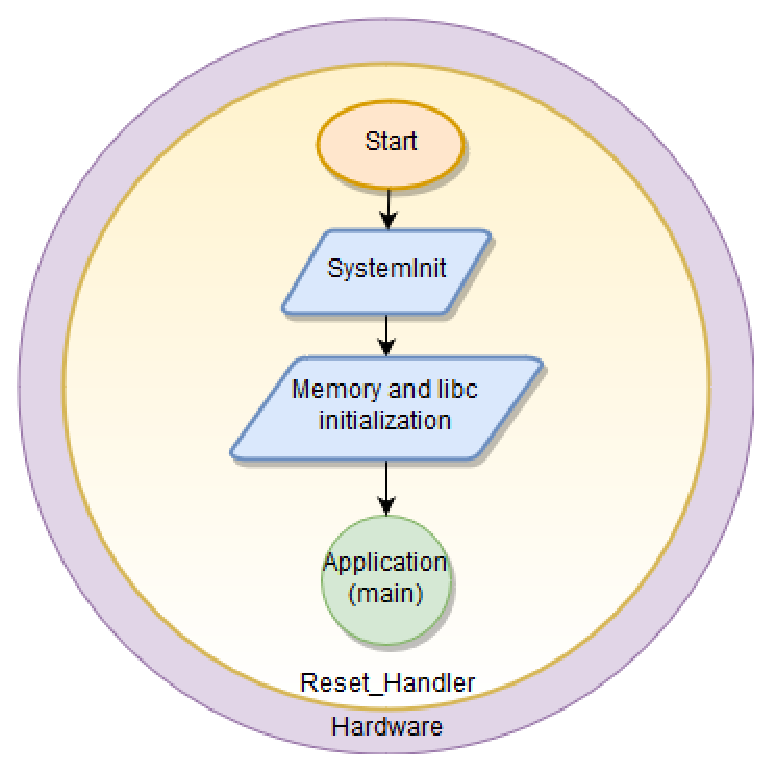
\includegraphics[width=0.75\textwidth]{initSeq}
    \caption{The initialization sequence of an MCU}
    \label{initSeq}
\end{figure}

\section{Implementing the bootloader}
In the following part we're going to present the technical details of how the bootloader and the helper tools, such as the Bundler and the Flasher are implemented.

As stated briefly in the previous part of this paper, there are three main components:

\begin{itemize}
\item the bootloader: an embedded application, which is responsible with managing the microcontroller and receiving the third party firmware file from the serial port. After the firmware is decrypted and loaded, it will be executed.
\item the Flasher tool: a PC application, that will be run by the client whenever he wants to change the application on the microcontroller. This tool is responsible with sending the bundled application (the firmware file) to the microcontroller using the serial port.
\item the Bundler tool: a PC application (available only to developers) that allows one to create firmware files for the microcontroller. The firmware files are encrypted and only the bootloader may decrypt them. The reason behind this decision was the fact that a potential cracker may intercept a firmware file and try to reverse engineer its mechanisms and thus, compromising the security of the embedded device.
\end{itemize}

So in order to maintain security we're going to need to encrypt and decrypt the firmware file. For this job, the symmetric key algorithm Rijndael was chosen, due to its unbroken security \cite{AES}. This algorithm is also known as the Advanced Encryption Standard, since it is used by the United States as a standard for encrypting communications \cite{wikiAES}.
The Rijndael algorithm requires the use of an encryption and decryption key. In order to maintain the security of the firmware file, this key should only be known to the Bundler tool and the bootloader, hence we're going to present how the bootloader and the keys will be laid out in the flash memory of the microcontroller.

\subsection{Memory Map}
The memory map of the microcontroller represents how the application code and data is laid out in memory. What starting address do they use, and how much space do they occupy.

In order to accomplish all of our goals, the memory will be split in three main sections, the bootloader's code which is the main part of this paper, the encryption keys, which will satisfy the security requirement and finally the user's application which will be decrypted and executed by the bootloader.

For exemplification and testing purposes we chose the MKV58F1M0VLQ24 microcontroller, based on the Cortex M7 ARM core. The microcontroller MKV58F1M0VLQ24 defines its memory map starting with address 0x10000000, this is also the address the bootloader is located at \cite{kv5x}.

The memory is divided into the three main sections as the following table shows:
\begin{table}[h]
\begin{tabular}{ | c | c | }
        \hline
       \textbf{Address} & \textbf{Description} \\ \hline
0x10000000 & Bootloader’s start address \\ \hline
0x10008000 & Encryption keys start address \\ \hline
0x1000a000 & Application start address \\ \hline
    \end{tabular}
        \centering
    \caption{The microcontroller's memory map}
    \label{protoStruct}
\end{table}

So the bootloader’s size is limited to maximum 32KB (including interrupt vector table and flash config), while the keys may span at most 8KB. The application may span the rest of the space up to the end of the flash memory (1MB – 40KB).
The keys are required to span a whole sector on the flash since we need to delete it when the keys are changed.
The linker scripts or scatter files of the application have to be modified according to the memory map required by the bootloader, ie. the applications should be placed in memory at 0x1000a000, otherwise they will not be loadable by the bootloader.

Also applications should not write the flash memory between address 0x10000000 and 0x1000a000, otherwise the device is recoverable only via a traditional re-flash, using a JTAG connector.

Please note that if the microcontroller is changed, the memory map and possibly the sector size will change too. That will lead to different starting positions and sizes of the application and the keys.

\subsection{The Bundler tool}
The Bundler tool is responsible with converting the application executable file (the result of the compilation process) to the firmware file that can be used by the Flasher tool to send to the bootloader. Basically it takes the output of the compilation process (the \texttt{.bin} file), encrypts it using an encryption key and writes it back in the \texttt{.fw} file format. The resulting \texttt{.fw} file is the one that the flasher will use to feed the bootloader.
Generally the embedded compilers generate the executable file in the \texttt{.hex} format \cite{hex}. In order to generate a \texttt{.bin} file from a \texttt{.hex} file you can use \texttt{srec\_cat} \cite{srecord}:
\begin{verbatim}
srec_cat file.hex -intel -offset - -minimum-addr file.hex -intel -o file.bin -binary 
\end{verbatim}

If you have the binary file and a key file, an example command for running the Bundler is:
\begin{verbatim}
bundler.exe keys\xyz.key app\Debug\app.bin
\end{verbatim}

After this command runs, we should end up with a \texttt{app.fw} file in the \texttt{app\textbackslash Debug\textbackslash} directory that is suitable for usage with the Flasher tool.
Please note that the Bundler only takes two arguments and the order is not relevant. One argument should be the path to the \texttt{.key} file and the other one should be the path to the application's \texttt{.bin} file.

\subsection{The Key files}
If you need to generate a new key file, the process is simple (on Linux):
\begin{verbatim}
head -c 16 /dev/urandom > keys/xyz.key
\end{verbatim}

The key files are simple binary files, of size 16 bytes. The 16 bytes represent the key that the Bundler will use to encrypt the \texttt{.bin} application with and then store it in the firmware file. It is important that the key used by the Bundler is also the key the bootloader will also use to decrypt the firmware, otherwise the flashing process will fail.

\subsection{The Flasher tool}
The Flasher tool is used to load a new application on the bootloader enabled MCUs. This is done by sending a firmware bundle to the microcontroller by means of serial communication. The firmware should be received by the client from the developers.

A prerequisite of using the Flasher tool is to first connect the microcontroller and the personal computer using a serial cable and determining the serial port on the PC the cable is connected to. On Windows based machines this can be done by inspecting the \texttt{Ports (COM \& LPT)} section of the \texttt{Device Manager}. The port should look like: COM4.

After the bootloader is started, the client has approximately 20 seconds to properly start the Flasher tool.
For the loading to be successful the user needs to use the COM port determined earlier and the path to the firmware file received from the application's developers.
In order to run the Flasher tool a command window has to be opened, then the following command has to be run:
\begin{verbatim}
flasher.exe -p COM4 path\to\app.fw
\end{verbatim}

The Flasher takes exactly two arguments, a named one and a positional one:
\begin{itemize}
\item \texttt{-p COM4}: represents the communication port
\item \texttt{path\textbackslash to\textbackslash app.fw}: this is the path to the firmware file the client received from the developers. This file was created using the Bundler tool.
\end{itemize}

\subsection{The Bootloader}
Having to deal with reading a firmware file from the serial port, decrypting it, writing it to the flash memory and loading it, the bootloader is divided into several functional modules that each handle some independent responsibility. The modules will then be combined together in order to achieve the desired functionality: loading a third party application in a secured way.

The architecture of the bootloader may be seen in figure \ref{architecture}.

\begin{figure}[h]
    \centering
    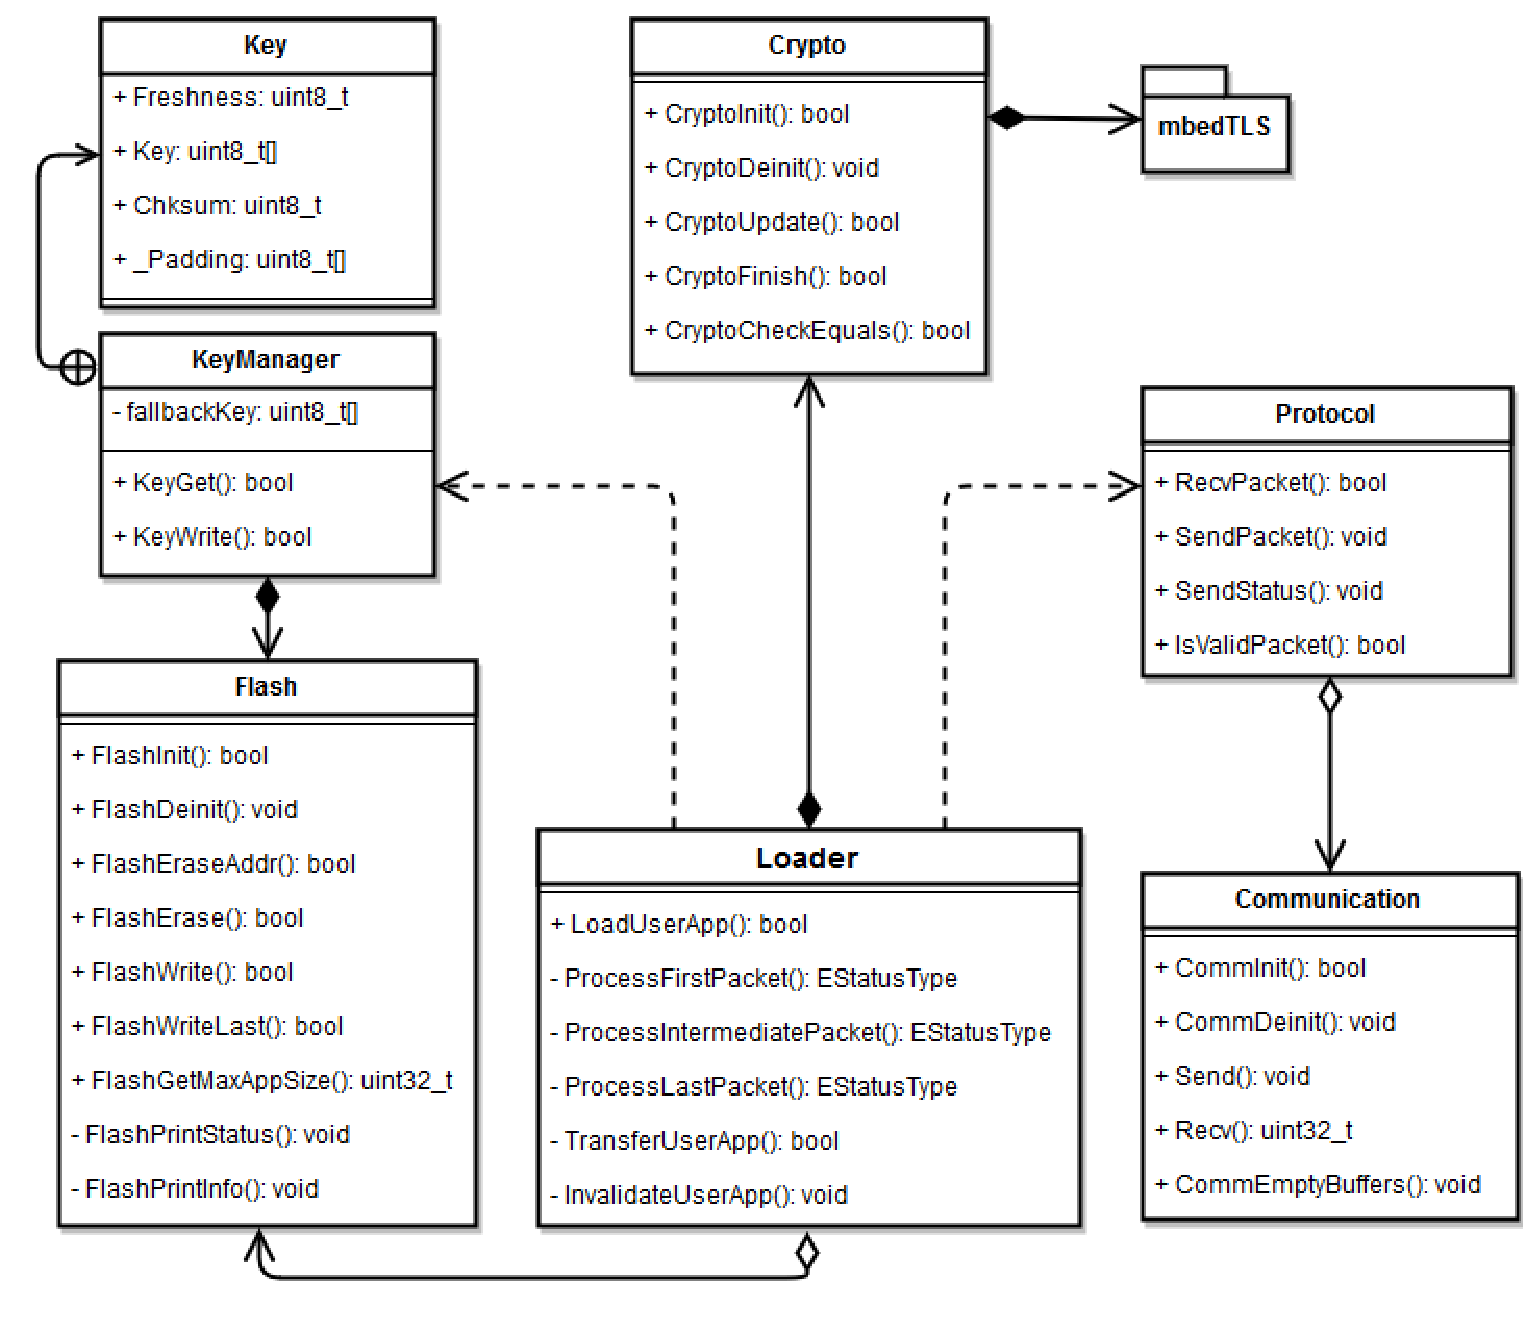
\includegraphics[width=1\textwidth]{arhitectura}
    \caption{The bootloader's modular architecture}
    \label{architecture}
\end{figure}

In this figure we can distinguish the following modules and responsibilities:
\begin{itemize}
\item \textbf{Flash}: This module is used for writing, reading and erasing the flash memory of the microcontroller.
\item \textbf{Crypto}: Its role is to manage the cryptograpy library and to provide an abstraction layer over it. The library used here is called \texttt{mbedTLS} and it implements the Rijndael algorithm used to encrypt and decrypt the user application.
\item \textbf{Communication}: Implements the communication channel, it is responsible with opening the serial port, sending and receiving of data and of course is also responsible of properly closing the port.
\item \textbf{Protocol}: It packages and formats the data in packets in order to facilitate the communication.
\item \textbf{KeyManager}: Responsible for writing and reading the encryption keys in their reserved memory areas.
\item \textbf{Loader}: This is the module that brings all the other functionality together and performs the actual application loading on the microcontroller.
\end{itemize}

The most complex module of all is the \texttt{Loader} module, which combines all the other functionality in order to transfer the application on the serial port, decrypt and execute it. Figure \ref{loaderStates} shows how the module works on a high level.

\begin{figure}[H]
    \centering
    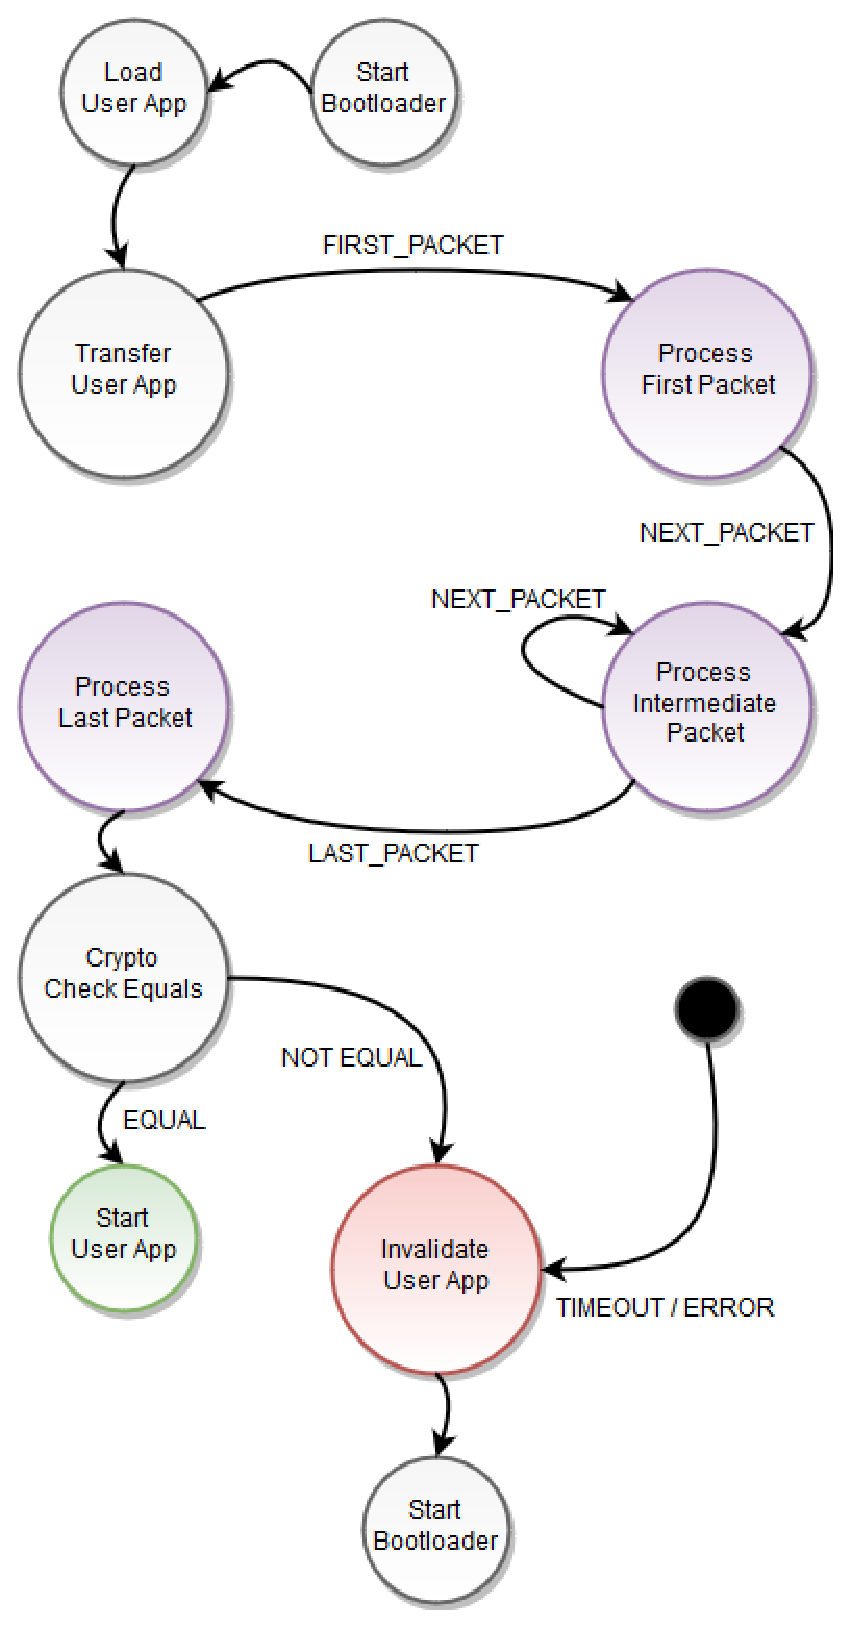
\includegraphics[width=0.7\textwidth]{loader_states}
    \caption{The data flow in the \texttt{Loader} module}
    \label{loaderStates}
\end{figure}

This data flow is based on the protocol developed specially for the bootloader, the transitions between states are determined by the arrival of different packet types:

\begin{itemize}
\item \textbf{FIRST\_PACKET}: The first packet sent from the Flasher to the bootloader. After this packet only packets of type \texttt{NEXT\_PACKET} will follow.
\item \textbf{NEXT\_PACKET}: An intermediary packet neither the first, nor the last. The number of these packets sent by the Flasher and received by the bootloader vary with the application's size, the bigger the application, the more packets sent to the bootloader.
\item \textbf{LAST\_PACKET}: This type of packet always follows a \texttt{NEXT\_PACKET} packet and is surely the last packet that the bootloader will receive.
\end{itemize}

The states of the \texttt{Loader} module represent functions inside the code, these do the processing required after a state transition and hopefully will end up in the \texttt{StartUserApp} state, which means that the application was successfully transferred and decrypted and lastly it can be executed.

It should be noted that each of these modules are implemented in a source file, with the \texttt{.c} extension and a header file, with \texttt{.h} extension.

\subsection{The communication protocol}
As stated previously, there needs to be a standard way of communicating between the Flasher tool and the bootloader running on the microcontroller. This standard way is implemented by the means of a communication protocol. This protocol is implemented by the \texttt{Protocol} module of the bootloader, which is shared by the Flasher tool, too.

The packet structure of the protocol may be seen in the table \ref{protoStruct}.

\begin{table}[h]
    \begin{tabular}{ | c | c | c | c | }
        \hline
        \textbf{Zone} & \textbf{Address} & \textbf{Description} & \textbf{Size (bytes)} \\ \hline
        \multirow{3}{*}{Header} & \texttt{0x00} & ID (fixed at 0xA5A5) & 2 \\ \cline{2-4}
                               & \texttt{0x02} & Type of packet & 1 \\ \cline{2-4}
                               & \texttt{0x03} & Length & 1 \\ \hline   
        Data                   & \texttt{0x04} & Content of packet & variable \\ \hline
        CRC                    & - & Polynomial code & 2 \\ \hline
    \end{tabular}
    \centering
    \caption{Packet structure for the communication protocol}
    \label{protoStruct}
\end{table}

Apart from the fixed ID that starts a packet, the type of packet field may take several values. These values were presented in the last section of this document and in addition to those, there is one more packet type, \texttt{STATUS\_PACKET} that has the role of communicating the status of the transfer up to this point in time.
After the type of the packet, the length field follows, which indicates how many data bytes of the application will be sent from the Flasher to the bootloader in the current packet. After the actual data, a 16 bit CRC is appended to the end of the packet in order to make sure the transmission of the packet is done without errors.

The message sequence diagram in figure \ref{protocol-msd} illustrates the process of successfully sending a firmware file from the Flasher tool to the bootloader.

\begin{figure}[H]
    \centering
    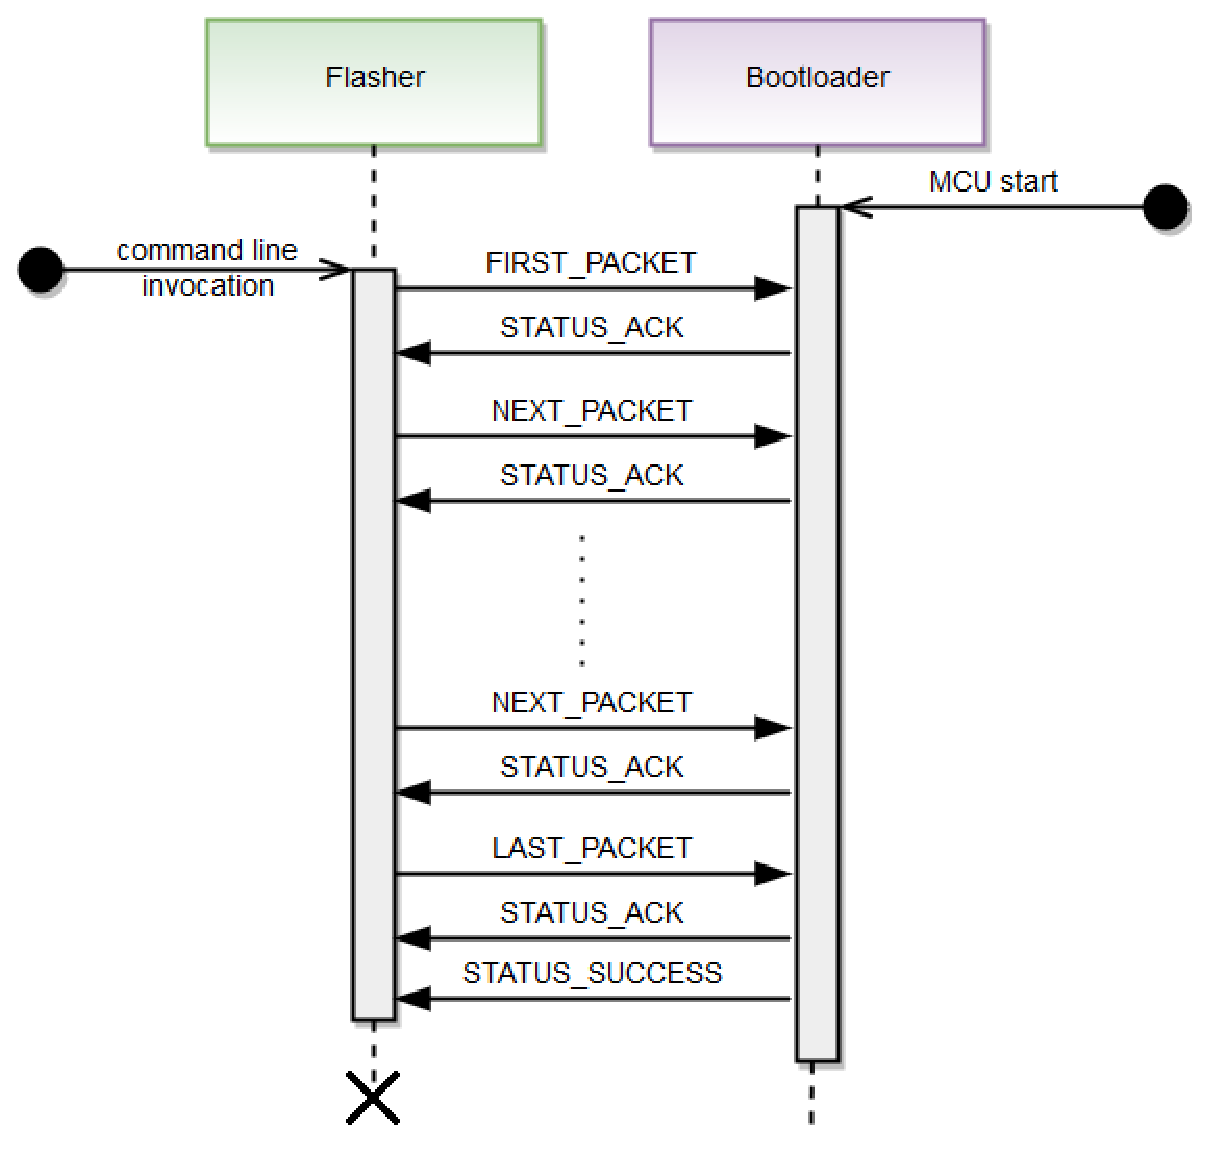
\includegraphics[width=1\textwidth]{protocol-en}
    \caption{Protocol message sequence diagram}
    \label{protocol-msd}
\end{figure}

It can be seen in this figure that the transfer stars when both the Flasher and the bootloader are ready to send and receive data and the fact that every packet is followed by a \texttt{STATUS\_PACKET} indicating that the transfer up to a certain point was successful.

The last two packets are sent by the bootloader, acknowledging the receipt of the last packet and indicating the success of the whole transmission of the firmware file.
After the firmware file was successfully transmitted, the bootloader proceeds with executing the third party application.

\section{Conclusions and future work}
This paper successfully presented the design and implementation of a bootloader for embedded devices. The aim of the bootloader was to allow for cost reductions security and flexibility of embedded applications deployment.

The cost reductions are achieved by allowing the users to program applications on the microcontrollers without the necessity for special programmer hardware. The flashing, when using the bootloader, can only be done using a serial cable connected to a personal computer. The flexibility comes from the fact that the bootloader allows the client to change the application on the microcontroller whenever there is an update available, without the need to ship the device to the developer so he can program it securely using the special JTAG connectors.

Although the practical implementation on the MKV58F1M0VLQ24 microcontroller was a success, there are still open points that may be improved.
One such point would be to allow the bootloader to write multiple applications into the flash memory, given the fact that enough storage space is available.
Also the usability of the Bundler and Flasher tools can be improved by implementing a Graphical User Interface, since now they are console based programs.
Finally, the portability of the bootloader may be enhanced to other microcontrollers in the future, this task is made simple by the fact that all the modules are written independently. Partly this feature was demonstrated by the fact that the Flasher tool shares the same protocol code with the bootloader, no line of code had to be changed for it to work.

\section{References}
\begin{thebibliography}{*}\label{Refences}
\bibitem{jtag}
Wikipedia, \newblock JTAG \newblock {\em https://en.wikipedia.org/wiki/JTAG}, Accessed March 2017. \vspace{-7pt}

\bibitem{bootstrapping}
Wikipedia, \newblock Bootstrapping \newblock {\em https://en.wikipedia.org/wiki/Bootstrapping\#Etymology}, Accessed March 2017. \vspace{-7pt}

\bibitem{kv5x}
NXP Semiconductors, \newblock {\em KV5x Sub-Family Reference Manual}, June 2016, \newblock Revision 4.\vspace{-7pt}

\bibitem{AES}
Joan Daemen and Vincent Rijmen, \newblock {\em The design of Rijndael: AES — the
Advanced Encryption Standard}, 2002, \newblock Springer-Verlag. \vspace{-7pt}

\bibitem{wikiAES}
Wikipedia, \newblock Advanced encryption standard \newblock { \em https://en.wikipedia.org/wiki/Advanced\_Encryption\_Standard}, Accessed February 2017. \vspace{-7pt}

\bibitem{srecord}
Peter Miller, \newblock Srecord - Binary Files \newblock {\em http://srecord.sourceforge.net/man/man1/srec\_examples.html\#BINARY\%20FILES}, Accessed February 2017.\vspace{-7pt}

\bibitem{hex}
ARM Group, \newblock General: Intel Hex File Format \newblock {\em http://www.keil.com/support/docs/1584/}, Accessed February 2017.\vspace{-7pt}

\end{thebibliography}

\vspace*{1cm} {\footnotesize
\begin{tabular*}{16cm}{p{4.2cm}p{4.2cm}p{4.2cm}}
Barbu Paul - Gheorghe & & \\
"Lucian Blaga" University of Sibiu &  &  \\
Department of Computer Science and Electrical Engineering &  & \\
 10 Victoriei Bd., Sibiu 550024 & & \\
ROMÂNIA & & \\
E-mail: \ {\it barbu.paul.gheorghe@gmail.com}& &

\end{tabular*}}

\end{document}
